In this chapter, we have applied both of the previously presented absolute and difference-based extrapolation frameworks to the nucleus \n{6}{Li}. For that, we have simulated a real use-case scenario by using NCSM calculations up to $N_\mathrm{max} = 10$.

Using the observations obtained from the \n{6}{Li}, we can decide on a final choice for the training mode and framework, which will be used to produce a final prediction for the \n{6}{Li} nucleus.

Now that we have applied the different training modes and the two framework to a real use-case, we are ready to formulate our final verdict about the frameworks as well as the training modes. For the training modes, we have already formulated two conditions that are necessary. They have to provide more reasonable predictions than the unmodified training mode and be consistent. In the previous chapters, we have seen that the $N_\mathrm{max}$-limitation training mode yielded inconsistent predictions for three training nuclei. This conforms to our observations in the evaluation of \n{6}{Li}, where the training mode produced reasonable but inconsistent results. The SRG-filter training mode was deemed the most promisable one in the evaluation of the three training nuclei. Unfortunately, this training mode resulted in the predictions of very unreasonably high values for the \n{6}{Li} nucleus.

Each of the training modes provided good results in some cases, but worse results than the unmodified training in other cases. Based on this inconsistency, we decide that the unmodified training mode is the most stable across all different scenarios, which is why we will be using this mode in our final result for \n{6}{Li}.

Now we come to a verdict about the two different extrapolation frameworks. The first framework consisted of the extrapolation of sequences of absolute energy values, while the second framework consisted of extrapolating difference sequences. While we observed that the difference-based framework produced a little smaller uncertainty for \n{6}{Li}, we saw in the previous chapters \ref{chap:extended} and \ref{chap:diff}, that the difference-based framework produced more reasonable predictions and generally smaller uncertainties as the absolute-based framework. For that reason, we decide on the difference-based framework as the generally better method of extrapolating ground-state energies.

Using the difference-based framework as well as the unmodified training process, we can state a final extrapolation result for the \n{6}{Li} nucleus. Since we have two maximum $N_\mathrm{max}$ values available, we have to decide on one for the final extrapolation. In a real use-case, one would decide on the maximum $N_\mathrm{max}$ available in order to input the maximum amount of information about the sequence limit into the network, as the higher $N_\mathrm{max}$ values are more converged. Using this, we decide on the extrapolation result of $N_\mathrm{max} = 10$ as the final prediction of the \n{6}{Li} ground-state energy value, which is given by \SI{-32.976 \pm 0.329}{\mega\electronvolt} for the interaction evolved with a flow parameter of \srg{0.04} and \SI{-32.542 \pm 0.272}{\mega\electronvolt} for the flow parameter of \srg{0.08}. The histograms of those extrapolations can be found in \autoref{fig:hists_li6}.

For the computation of the final prediction, as well as the error estimate, we assumed that the network prediction are normally distributed. The distribution of the predictions for the flow paramter $\alpha$ of \srg{0.04} show a good compliance to the shown normal distribution. However, we also see that the distribution is slightly skewed towards lower energy values. This effect is amplified in the distribution of predictions for $\alpha = \srg{0.08}$, where there is a sharp decline in predictions for high energies bigger than \SI{-32.1}{\mega\electronvolt}, but a higher amount of predictions for lower energies. As a result, the assumption of a normal distribution leads to a lower prediction than the most guessed value. To generate a more meaningful prediction and uncertainty, we could assume a probability density that takes this skewness into account.

\begin{figure}[H]
  \begin{subfigure}{.5\textwidth}
    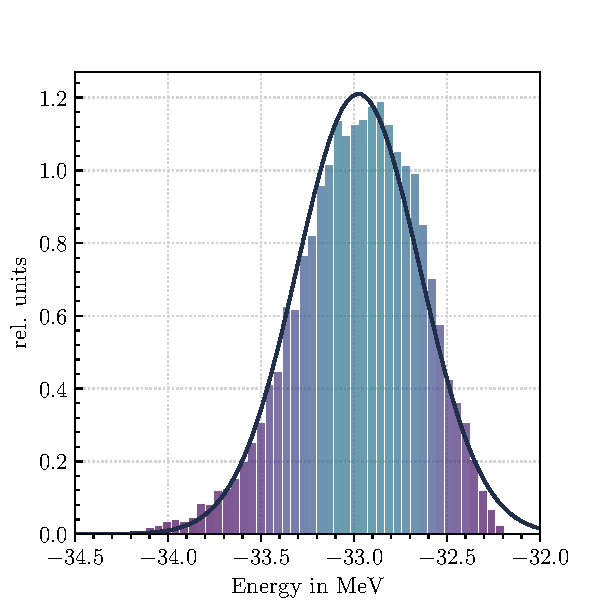
\includegraphics[width=\textwidth]{media/li6_0400_histogram.pdf}
    \caption{}
  \end{subfigure}
  \begin{subfigure}{.5\textwidth}
    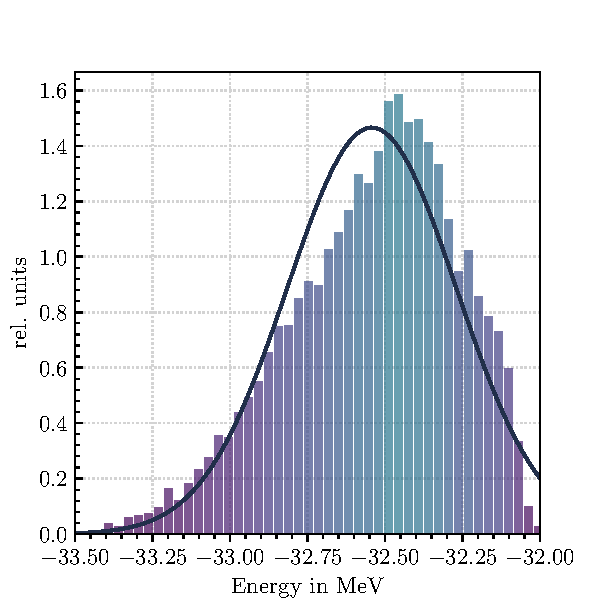
\includegraphics[width=\textwidth]{media/li6_0800_histogram.pdf}
    \caption{}
  \end{subfigure}
  \caption{Histograms for the final extrapolation of \n{6}{LI} for the different SRG flow parameters of \srg{0.04} \textbf{(a)} and \srg{0.08} \textbf{(b)}. The bar heights have been normed such that the total area of them is 1. The final extrapolation used the difference-based framework together with an unmodified training process.}
  \label{fig:hists_li6}
\end{figure}
